\section{Near Detector}\label{sec:nu-osc-06}\label{sec:physics-lbnosc-ND}

% NOTES
% This section must be consistent with the ND executive summary
% Details of the ND as implemented in the LBL analysis are in the appendix
% Section references ArgonCube paper, gas TPC public note
% Need DUNE-PRISM public note, or significant appendix on PRISM
% Need some details on gas TPC analysis in appendix

Oscillation parameters are determined by comparing observed charged-current event spectra at the \dword{fd} to predictions from simulation. These predictions are subject to uncertainties on the neutrino flux and cross sections at the level of tens of percent, as described in the preceding sections. To achieve the required few percent precision of \dword{dune}, it is necessary to constrain these uncertainties with a highly capable suite of \dwords{nd}.

The broad \dword{nd} concept is described in Section~\ref{sec:ndconcept}, along with an outline of the \dword{nd}'s role in the oscillation analysis. The reconstruction and event selection is described in Section~\ref{sec:ndsimreco}. More detail can be found in Appendix~\ref{sec:nu-osc-12}. \dword{nd} and \dword{fd} uncertainties are discussed in Section~\ref{sec:physics-lbnosc-syst}.

\subsection{The Near Detector Concept}
\label{sec:ndconcept}

The \dword{dune} \dword{nd} system consists of a \dword{lartpc}
%liquid argon (LAr) time projection chamber (TPC)
functionally coupled to a magnetized \dword{mptdet},  %multipurpose tracking (MPT) detector, 
in an underground hall at \dword{fnal} 574 m from the neutrino beam source. The \dword{lartpc} is modular, with fully-\threed  pixelated readout and optical segmentation. These features greatly reduce reconstruction ambiguities that hamper monolithic, projective-readout \dwords{tpc}, and enable the \dword{nd} to function in the high-intensity environment of the \dword{dune} \dword{nd} site. For containment of hadron showers the active dimensions are at least $4 \times 3$ m in the directions transverse to the beam, and 5 m in the beam direction, giving a total mass of at least 84 tons. The \dword{lar} detector is movable, to facilitate measurements at both on-axis and off-axis positions.

The \dword{mptdet} sits immediately downstream of the \dword{lar} cryostat, in a magnetic field with a strength of at least 0.4 T. It consists of a \dword{gartpc} %gaseous argon TPC 
in a pressure vessel at 10 bar, surrounded by a granular, high-performance electromagnetic calorimeter. The \dword{nd} concept is described in detailrd in Appendix~\ref{sec:physics-lbnosc-ND-app} and in the Executive Summary.

The oscillation analysis includes \dword{nd} samples from both \dwords{lartpc} and \dwords{gartpc}. %liquid argon and gas argon TPCs. 
The \dword{lar} $\nu_{\mu}$ and $\bar{\nu}_{\mu}$ \dword{cc} samples are divided into \twod bins on neutrino energy and inelasticity. Additionally, a sample of neutrino-electron elastic scattering events is isolated and used as a direct constraint on the flux normalization. Gas \dword{tpc} samples are used to constrain exclusive cross sections and nuclear effects, leveraging the low threshold and excellent \dword{pid} of the gaseous detector. Off-axis measurements on \dword{lar} are used to directly constrain uncertainties in energy reconstruction resulting from unmodeled detector and interaction uncertainties.

\subsection{Event Simulation and Parameterized Reconstruction}
\label{sec:ndsimreco}

Neutrino interactions are simulated in the active volumes of the \dword{lar} and \dword{hpg} \dwords{tpc}. The neutrino flux prediction is described in Section~\ref{ch:osc-bm-nus}. Interactions are simulated with the \dword{genie} event generator using the model configuration described in Section~\ref{sec:nu-osc-05}. The propagation of neutrino interaction products through the detector volumes is simulated using a \dword{geant4}-based model. Pattern recognition and reconstruction software has not yet been developed for the \dword{nd}. Instead, we perform a parameterized reconstruction based on true energy deposits in active detector volumes as simulated by \dword{geant4}. This section gives a qualitative overview of the selection, which is described in detail in Appendix~\ref{sec:nu-osc-12}.

\subsubsection{Liquid Argon charged-current interactions}

Liquid argon events are selected from a central $6 \times 2 \times 3$~m$^{3}$~fiducial volume that excludes 50 cm around the edges of the detector and 150cm downstream, which is required for good containment of hadronic showers. Hadronic energy is estimated by summing visible energy deposits in the active \dword{lar} volume. Events are rejected when energy is observed in the outer 30 cm of the detector, which is evidence of poor hadronic containment. This leads to an acceptance that decreases with hadronic energy, as shown in the right panel of Figure~\ref{fig:NDreco}.

Electrons are generally contained in the \dword{lar} and are reconstructed calorimetrically. Muons are contained up to kinetic energies of $\sim$1 GeV, above which they typically exit the detector. Forward exiting muons will enter the magnetized \dword{mptdet}, where their momenta and charge sign are reconstructed by curvature. The acceptance is somewhat lower at large angles, as shown in the center panel of Figure~\ref{fig:NDreco}.

Events are classified as either $\nu_{\mu}$ \dword{cc}, $\bar{\nu}_{\mu}$ CC, $\nu_{e}$+$\bar{\nu}_{e}$ \dword{cc}, or \dword{nc} based on the presence of charged leptons. Backgrounds to $\nu_{\mu}$ \dword{cc} arise from \dword{nc} $\pi^{\pm}$ production where the pion leaves a long track and does not shower. Muons below about 400 MeV kinetic energy have a significant background from charged pions, so these \dword{cc} events are excluded from the selected sample. Backgrounds to $\nu_{e}$ \dword{cc} arise from photons that convert very near the interaction vertex. The largest contribution is from $\pi^{0}$ production with highly asymmetric decay.

\begin{dunefigure}[ND reconstruction]{fig:NDreco}
{Left: Reconstructed vs. true neutrino energy for $\nu_{\mu}$ \dword{cc} events with either contained or MPT-matched muon and ell-contained hadronic shower. The bin at zero true energy corresponds to events that are not true $\nu_{\mu}$ \dword{cc}, which are mostly neutral current with a charged pion faking the muon track, hence the lower energy spectrum. Center: Detector acceptance for $\nu_{\mu}$ \dword{cc} events as a function of muon transverse and longitudinal momentum. Right: Acceptance as a function of hadronic energy; the black line is for the full fiducial volume while the red line is for a $1 \times 1 \times 1$~m$^{3}$ volume in the center, and the blue curve is the expected distribution of hadronic energy given the \dword{dune} flux.}
 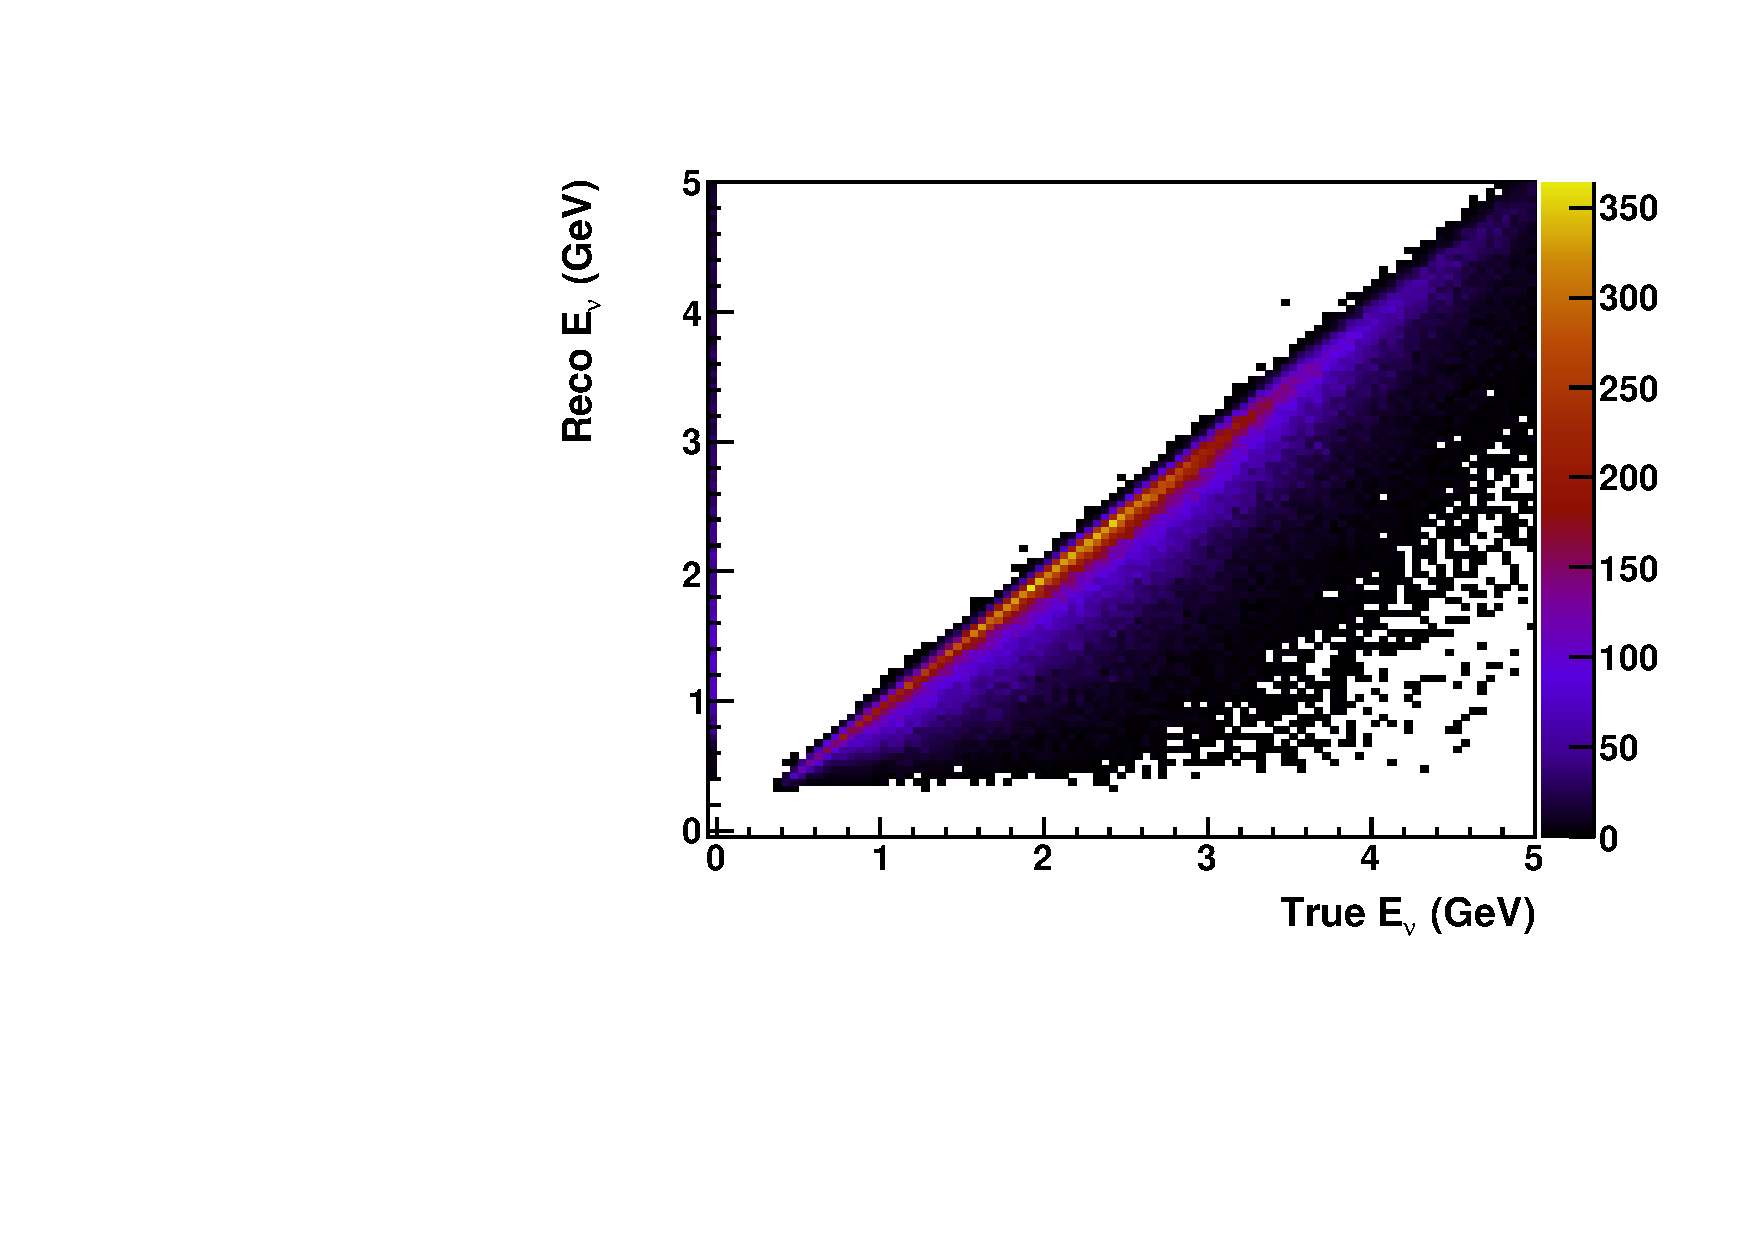
\includegraphics[width=0.3\textwidth]{true_reco_Ev.pdf}
 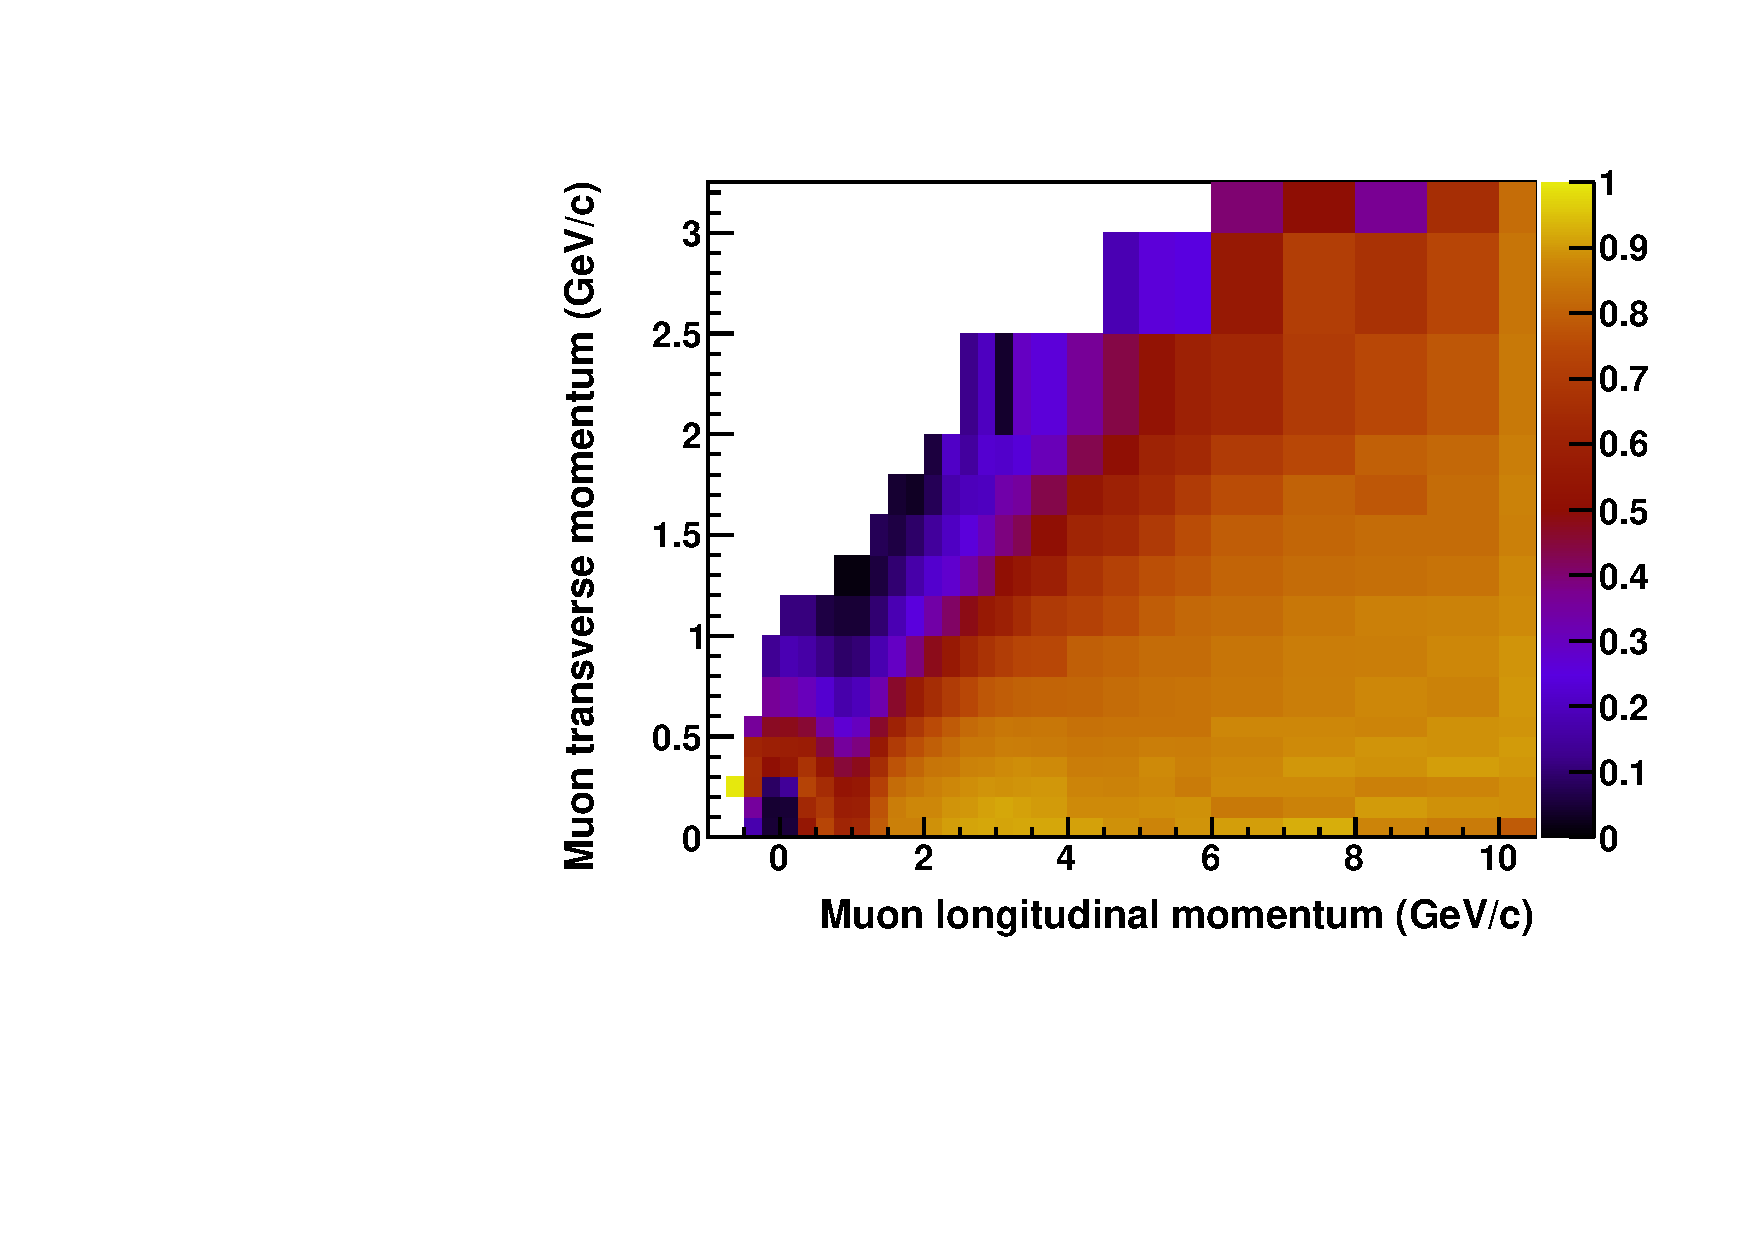
\includegraphics[width=0.3\textwidth]{pL_pT_eff.pdf}
 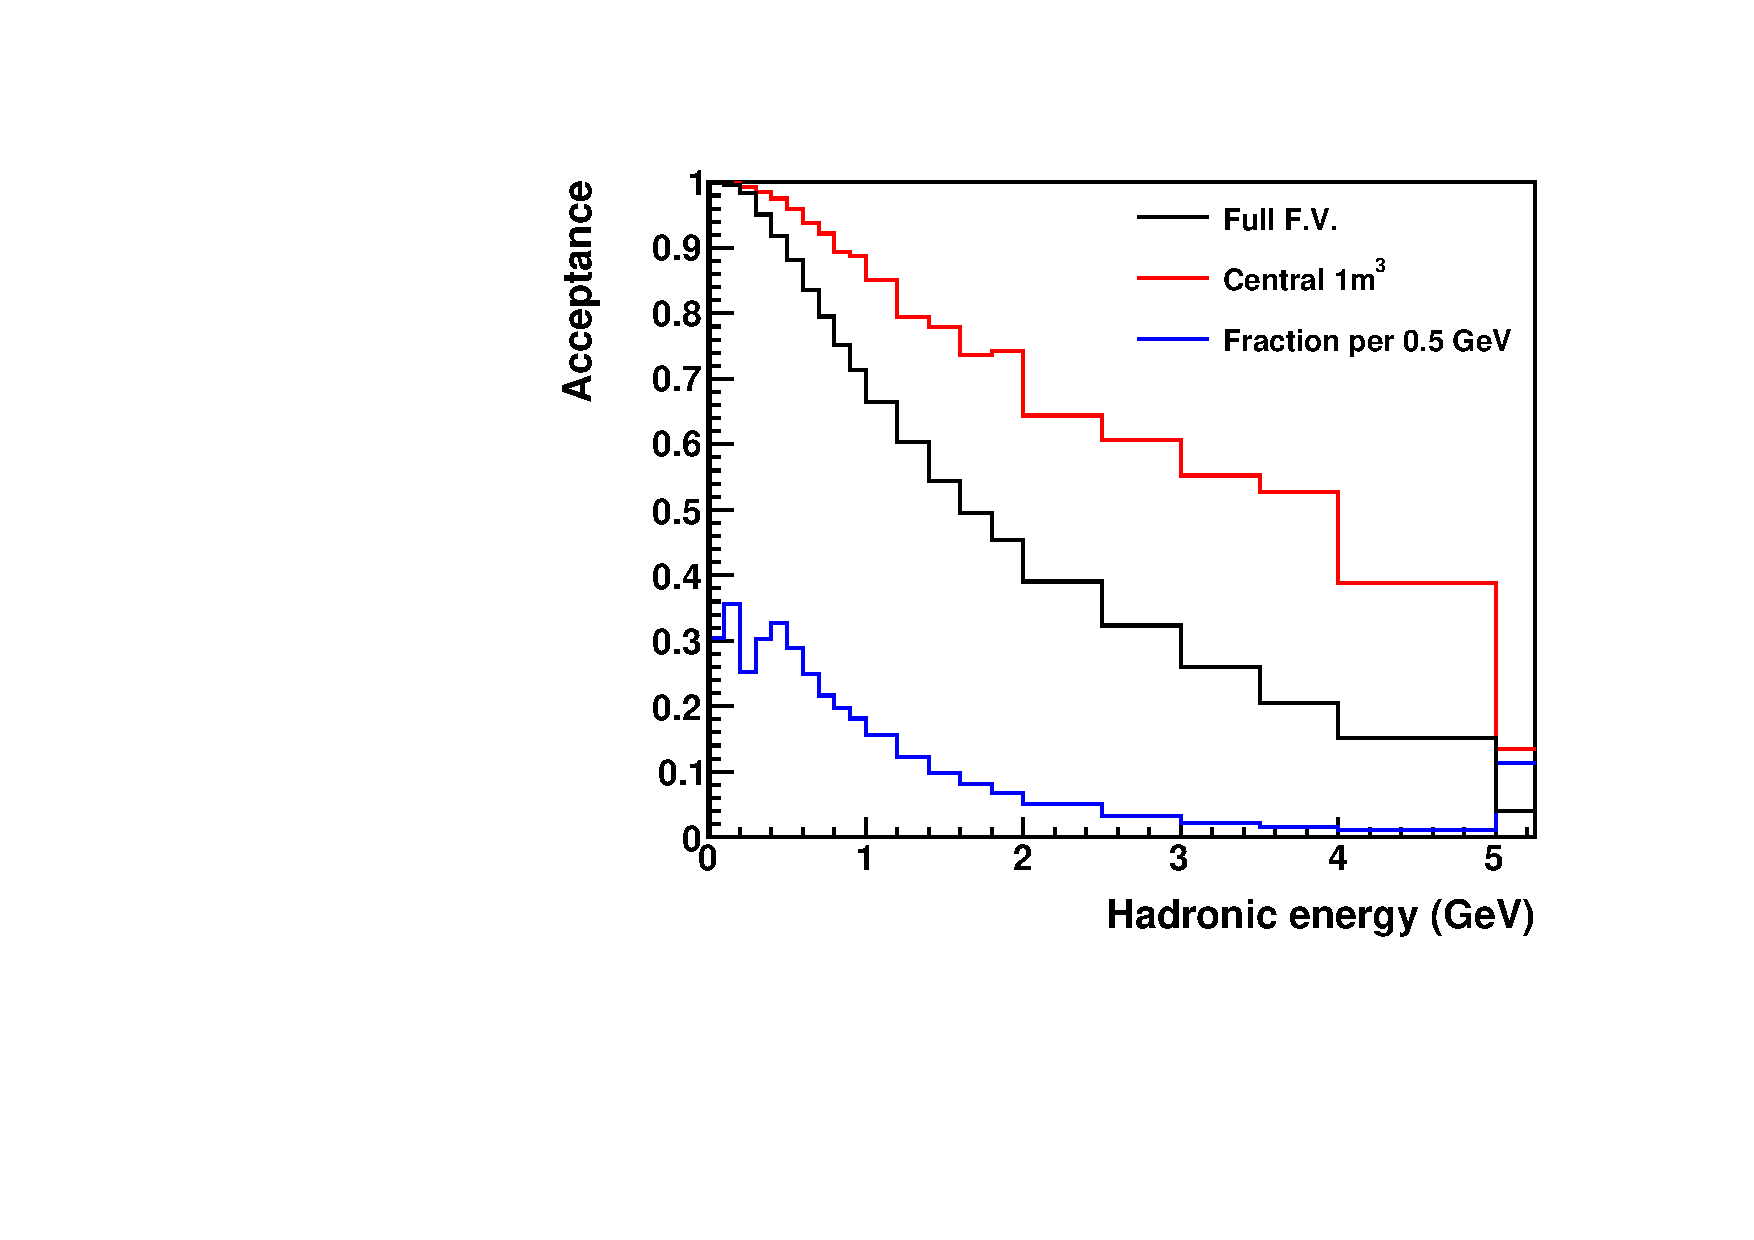
\includegraphics[width=0.3\textwidth]{Ehad_eff.pdf}
\end{dunefigure}

\subsubsection{Neutrino-electron elastic scattering}

Neutrino-electron scattering is a pure-electroweak process with calculable cross section at tree level. It is therefore possible to directly constrain the flux by measuring the event rate of $\nu+ e \rightarrow \nu +e$ and dividing by the known cross section. The two-body elastic process is subject to the kinematic constraint $E_{e}\theta_{e}^{2} < 2m_{e}$, where $E_{e}$, $\theta_{e}$, and $m_{e}$ are the final-state electron energy, angle, and mass, respectively.

The \dword{lartpc} has sufficient energy and angular resolution to separate the signal, peaked at low $E_{e}\theta_{e}^{2}$, from backgrounds due to $\nu_{e}$ \dword{cc} scattering and from \dword{nc} $\pi^{0}$ production. The expected rate is \num{3300} events per year, so that the statistical uncertainty on the absolute flux normalization can be constrained to $\sim$1\% with three years of running. The dominant systematic uncertainty is expected to be the $\nu_{e}$ \dword{cc} shape at low $Q^{2}$, and can be constrained with sidebands to the $\sim$1\% level so that the overall uncertainty is $\sim$2\%.

\subsubsection{Off-axis \dword{nd} measurements}
\label{sec:ch-nu-osc-06-ndconcept-offaxis}

Neutrino energy reconstruction is one of the biggest challenges in a precision long-baseline oscillation experiment like \dword{dune}. Even with a highly capable \dword{fd}, a fraction of the final-state hadronic energy is typically not observed. For example, neutrons may travel meters without interacting, and can exit the detector with significant kinetic energy. This missing energy is typically corrected with a neutrino interaction generator, which is used to relate the true neutrino energy to the observed energy. These models have many tens of uncertain parameters, which can be constrained by \dword{nd} measurements. However, there may be many different parameter combinations that adequately describe the \dword{nd} data. These degenerate solutions can extrapolate differently to the \dword{fd}, where the flux is significantly different, primarily due to oscillations. This can lead to biases in the fitted oscillation parameters, including $\delta_{CP}$, despite an apparently good quality of fit.

These biases can be partially mitigated by an on-axis \dword{nd} capable of making numerous exclusive measurements, including a direct flux measurement via neutrino-electron elastic scattering. However, the energy dependence of the interaction cross section and the bias in reconstructed neutrino energy cannot be measured in a single beam. To gain sensitivity to this physics, the \dword{lartpc} detector is movable, and the \dword{nd} hall is oriented to facilitate both on-axis measurements and measurements at positions up to 33 m off axis. The flux spectrum varies as a function of off-axis angle, peaking lower in energy as the angle is increased, as shown in Figure~\ref{fig:OAAFluxFigs}. As uncertainties in the flux prediction are strongly correlated across off-axis angles, off-axis measurements of reconstructed neutrino energy constrain cross section uncertainties and provide futher handles on possible degeneracies in the fit. By taking linear combinations of such measurements, it is possible to reproduce the predicted \dword{fd} oscillated flux for some set of oscillation parameters, and directly compare visible energy between \dword{nd} and \dword{fd} over essentially the same flux, and with greatly reduced model dependence. Figure~\ref{fig:nd_prism} shows the result of such a linear combination, overlaid with the \dword{fd} flux. The off-axis technique cannot reproduce the \dword{fd} flux tail. The lower $E_{\nu}$ bound is determined by the range of accessible off-axis angles; to cover the second oscillation maximum down to 0.5 GeV, measurements out to 33 m off axis are required.

\begin{dunefigure}[DUNE-PRISM fluxes]{fig:nd_prism}
{The predicted \dword{fd} flux (black), and a prediction made up of linear combinations of \dword{nd} fluxes (green).}
 % Possibly include figure from mock data study here
 %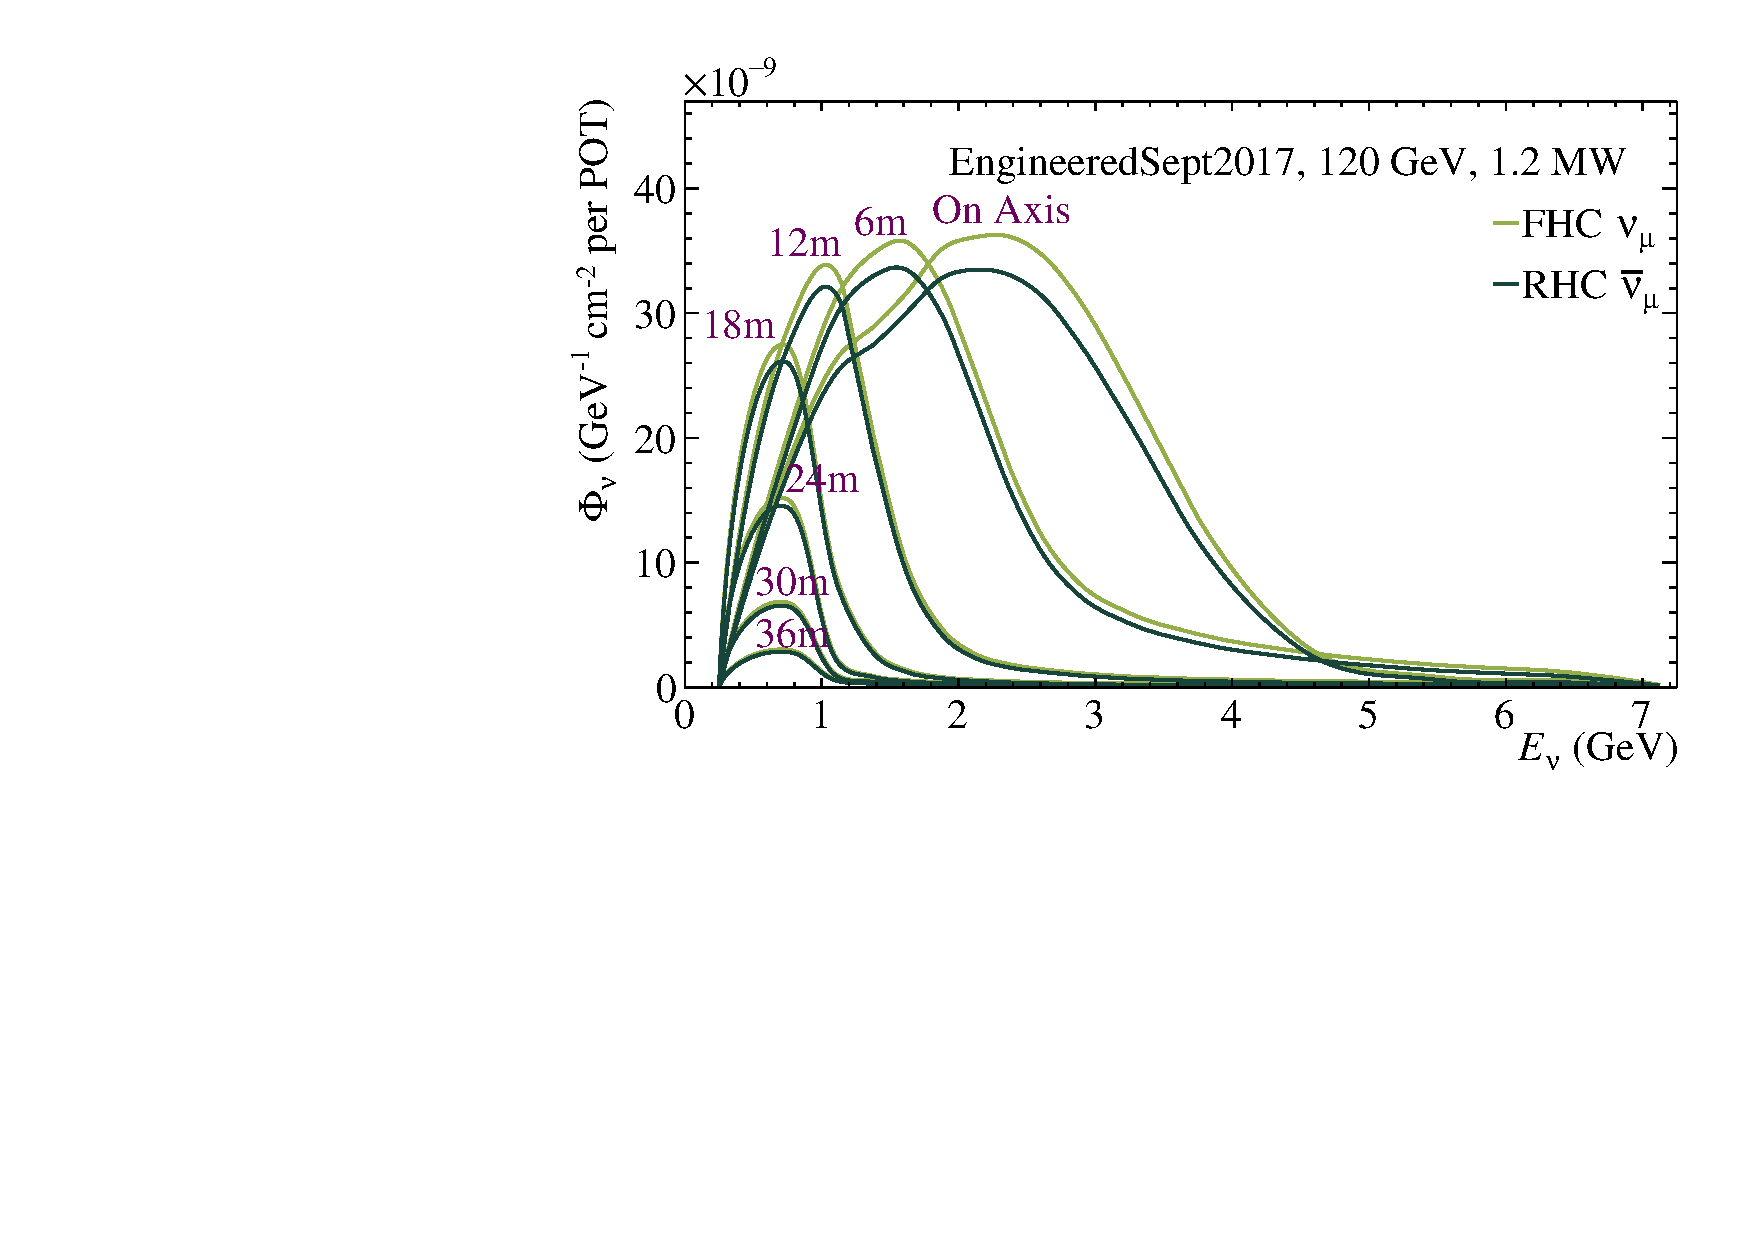
\includegraphics[width=0.49\textwidth]{graphics/OffAxisFluxes_1D.pdf}
 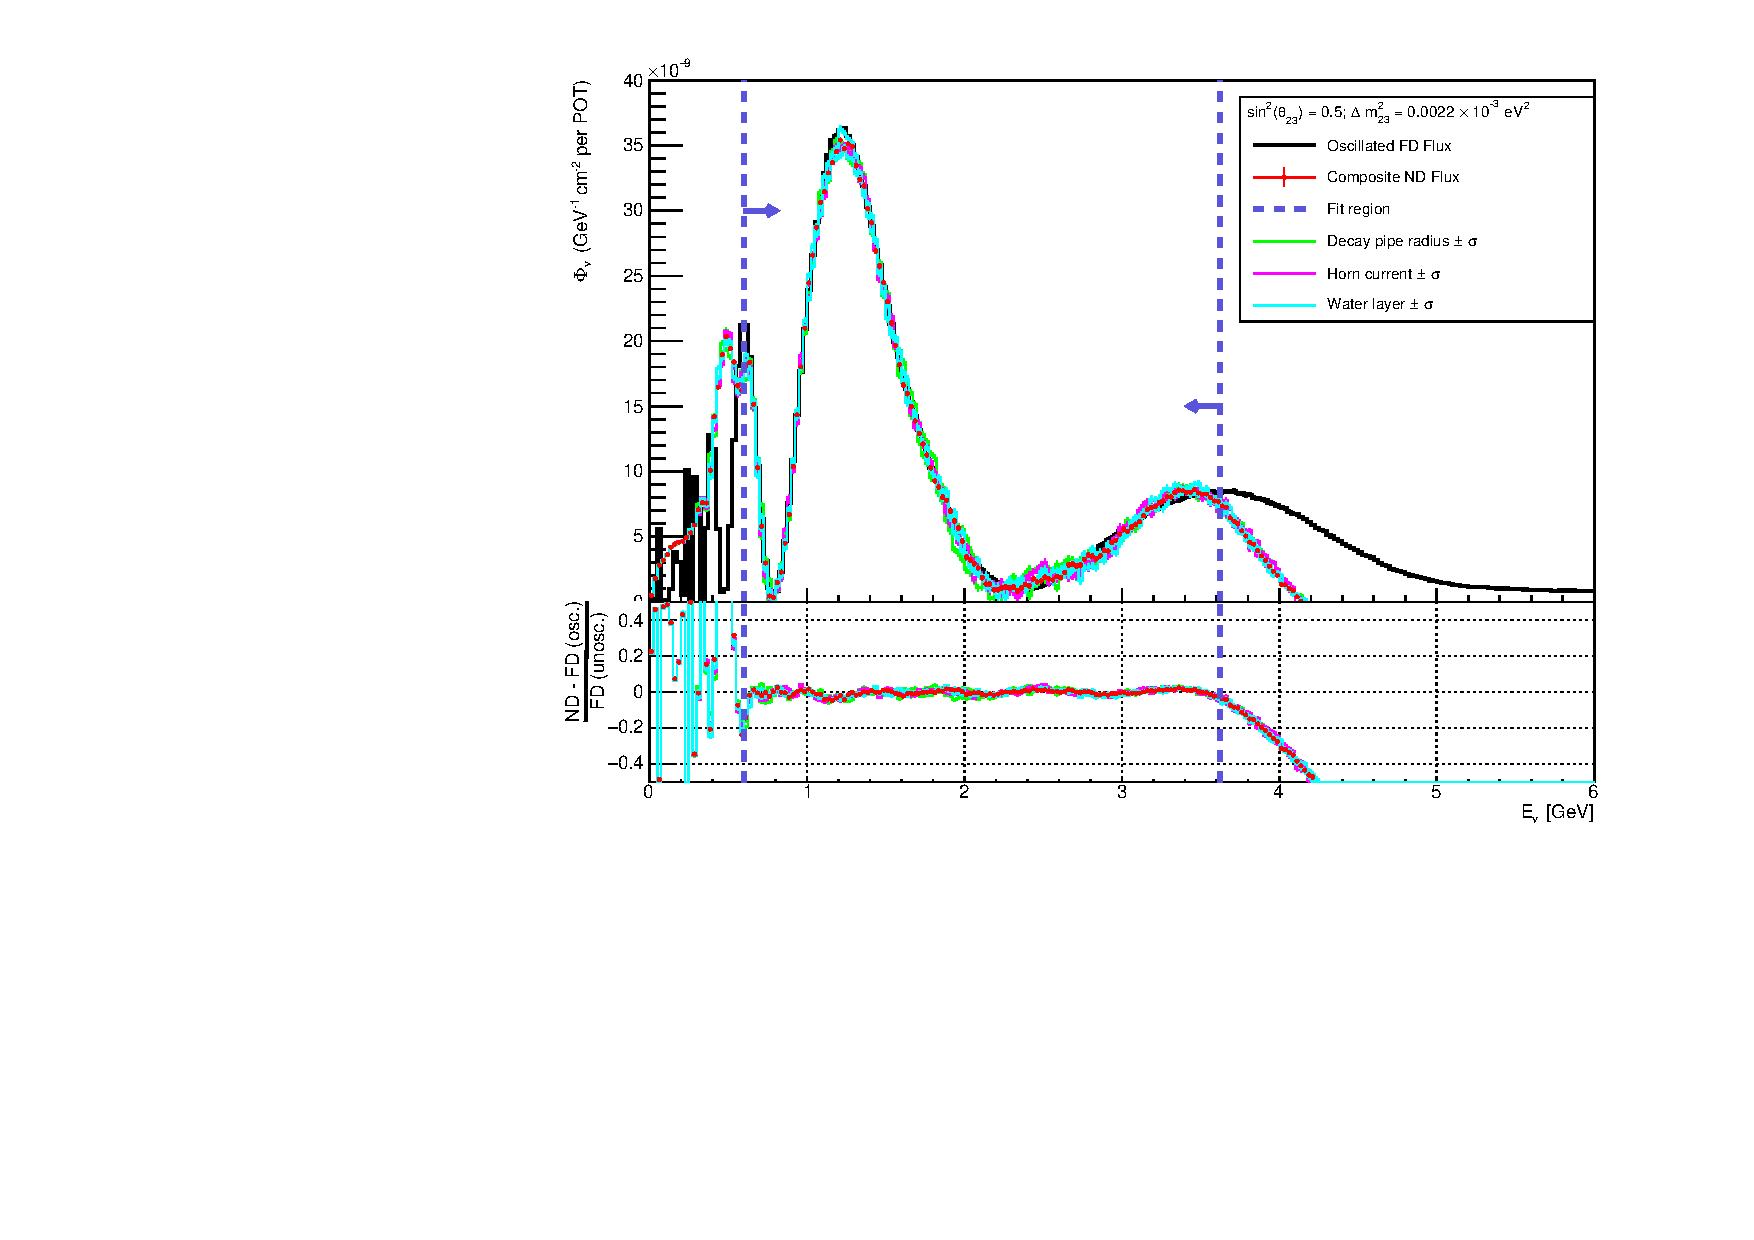
\includegraphics[width=0.49\textwidth]{graphics/nuprism_coef_oscSpectrum_0_0022_0_5.pdf}
\end{dunefigure}

A potential run plan is to take on-axis data approximately 50\% of the time, with the other 50\% split among enough off-axis positions so that the fiducial volumes of adjacent ``stops'' overlap, giving a continuous range of angles. Event selection at an off-axis location of the \dword{lar} detector is identical to the on-axis case. The selection efficiency varies as a function of muon energy due to containment and matching to the downstream magnetized tracker, and as a function of hadronic energy due to containment. As muon and hadronic energy are correlated to neutrino energy, the efficiency varies with off-axis position. The efficiency also varies as a function of vertex position; interactions occurring near the edges of the detector are more likely to fail containment requirements. These effects are corrected with simulation; as they are largely geometric, the uncertainties that arise from the corrections are very small compared to the uncertainties on neutrino cross sections and energy reconstruction. More details on the off-axis analysis are found in Appendix~\ref{sec:physics-lbnosc-ND-app}.

\subsubsection{Gaseous argon charged-current interactions}

With over 30 million charged-current events per year, the \dword{lartpc} event sample can be analyzed in many different exclusive channels and provide powerful constraints. However, its relatively high density makes certain hadronic topologies challenging to reconstruct. With its low reconstruction thresholds, excellent pion/proton separation, and charge reconstruction, the gaseous \dword{tpc} complements the \dword{lar} detector. In particular, measurements of proton and charged pion multiplicities as a function of neutrino energy constrain cross section uncertainties not accessible to the \dword{lar} alone.

In addition, the gas \dword{tpc} provides a useful check on the reconstruction efficiency of the \dword{lar} selection. Due to the combining of contained muons with gas \dword{tpc}-matched events, there are kinematic regions where the acceptance of the \dword{lartpc} is uncertain. Also, without a magnetic field, the wrong sign contamination cannot be directly measured, especially at high angle and low energy. The gas \dword{tpc}, however, has uniform acceptance over the full 4$\pi$, as well as charge measurement capability except when the muon is nearly parallel to the magnetic field lines.

Unlike the \dword{lartpc}, where the hadronic energy is determined by a calorimetric sum of energy deposits, the gas \dword{tpc} hadronic energy is reconstructed particle-by-particle, including pion masses. For this analysis, samples of $\nu_{\mu}$ \dword{cc} events are selected in slices of charged pion multiplicity, and fit as a function of reconstructed neutrino energy. The threshold for charged pion selection is 5 MeV, and $\pi^{+}$ can be reliably separated from protons up to momenta of 1.3 GeV/c.

